\chapter{実例研究}
本章では実例研究として、オーソドックスかつ単純な機能を持つキッチンタイマー(カウントダウンタイマー)の開発を行う。
これはソフトウェア的な複雑さを持つ小規模組込みシステムの典型的な例であり、SFRPが第一にターゲットとする類のシステムである。

\section{アプリケーションの仕様}
開発対象となるキッチンタイマー(KTIMER)の機能仕様を図\ref{fig:ktimer:spec}に簡単に示す。
この仕様に基づいて包括的な状態遷移図を作成すると図\ref{fig:ktimer:state}の様になる。

図\ref{fig:ktimer:state}において、四角形のテーブル3つがそれぞれアプリケーションの状態を表す。
各テーブルの1段目は状態名、2段目は状態変数の一覧、3段目はその状態におけるアプリケーションの動作を示している。
テーブル同士を繋ぐ矢印は状態遷移を表し、これに付属する文字列は遷移条件(角括弧の中)と遷移後の状態変数の値を示している。
また、左上に存在する中空からの矢印はアプリケーションの開始(停止状態からの遷移)を表している。


\begin{figure}[h]
\begin{screen}
\begin{itemize}
  \item 分と秒を2桁ずつ表示する表示器、ボタンA、ボタンB、ボタンC、ブザーを備える。
  \item 電源を投入すると、分数と秒数が共に0で一時停止した状態となる。
  \item 一時停止中にボタンCを押すとカウントダウンを開始する。ただし分数と秒数が共に0の場合は何もしない。
  \item 一時停止中にボタンAを押すと分数がカウントアップされる。ただし分数が99の場合は0に戻る。
  \item 一時停止中にボタンBを押すと秒数がカウントアップされる。ただし秒数が59の場合は0に戻る。
  \item 一時停止中にボタンAとBを同時に押すと分数と秒数が共に0にリセットされる。
  \item カウントダウン中にボタンCを押すと一時停止する。
  \item カウントダウンが0に達するとブザーが鳴る。
  \item ブザーが鳴っている時にボタンCを押すとブザーは停止し、分数と秒数が共に0で一時停止した状態になる。
\end{itemize}
\end{screen}
\caption{KTIMERの機能仕様}
\label{fig:ktimer:spec}
\end{figure}

\begin{figure}[h]
 \begin{center}
  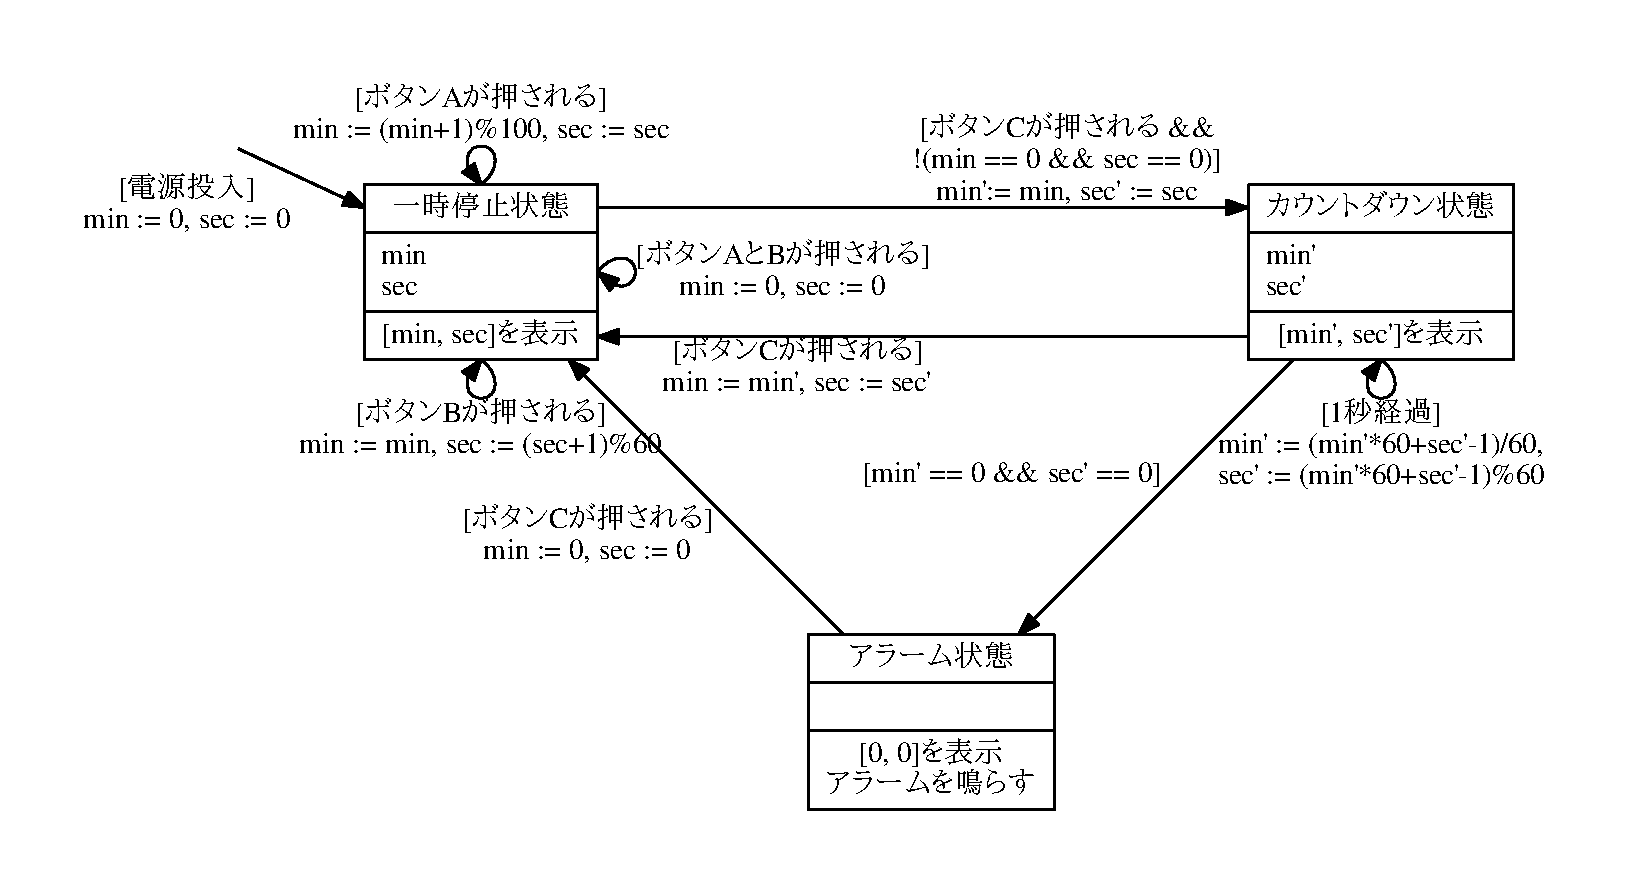
\includegraphics[width=155mm]{figure/ktimer_state.pdf}
 \end{center}
 \caption{KTIMERの状態遷移図}
 \label{fig:ktimer:state}
\end{figure}

\clearpage
\section{ハードウェア}
KTIMERのハードウェア仕様を図\ref{fig:ktimer:hardware}に簡単に示す。
この仕様に基づいてKTIMERの回路図を構成すると図\ref{fig:ktimer:circuit}の様になる。
図\ref{fig:ktimer:picture}はこの回路をブレッドボード上に実装した様子である。
実装に際し、電源電圧Vinの値はマイクロコントローラの動作電圧に合わせて5Vとした。
また、プルダウン抵抗R1の値は1k$\Omega$とし、制限抵抗R2の値は使用するLEDの最大許容電流との兼ね合いから200$\Omega$とした。

\begin{figure}[h]
\begin{screen}
\begin{itemize}
  \item マイクロコントローラにはAVR ATmega8を使用する。
  \item 時間の表示には4桁のカソードコモンの7セグメント表示器を用いてダイナミック点灯を行う。
  \item ボタンA、ボタンB、ボタンCにはそれぞれタクトスイッチを用いる。
  \item ブザーには圧電ブザーを用いる。
\end{itemize}
\end{screen}
\caption{KTIMERのハードウェア仕様}
\label{fig:ktimer:hardware}
\end{figure}

\begin{figure}[h]
 \begin{center}
  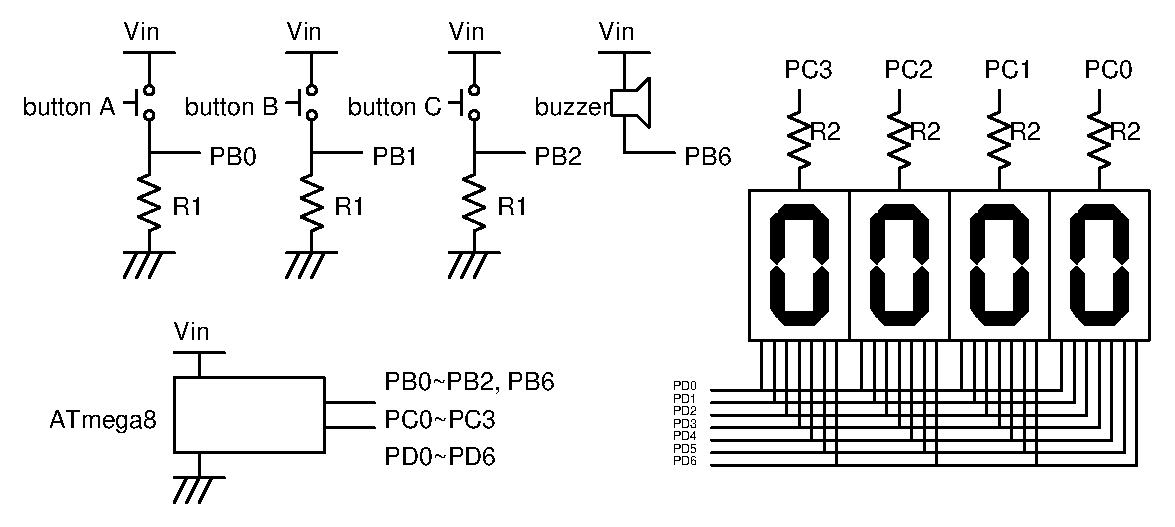
\includegraphics[width=160mm]{figure/circuit.ps}
 \end{center}
 \caption{KTIMERの回路図}
 \label{fig:ktimer:circuit}
\end{figure}

\begin{figure}[h]
 \begin{center}
  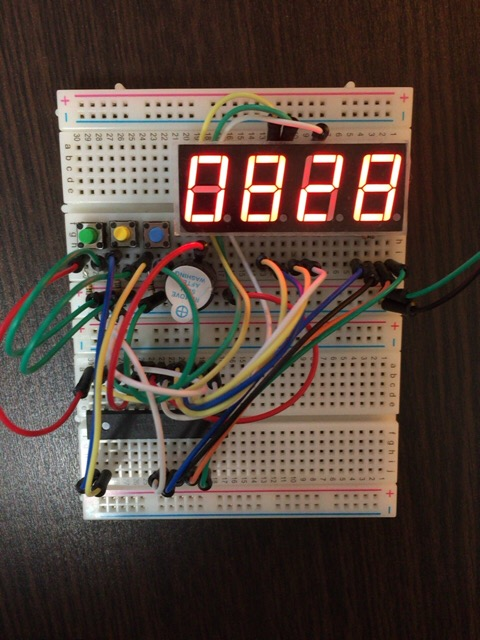
\includegraphics[scale=0.8]{figure/craft.jpg}
 \end{center}
 \caption{ブレッドボード上のKTIMER実装}
 \label{fig:ktimer:picture}
\end{figure}

\clearpage
\section{ソフトウェア}
Code \ref{code:ktimer:sfrp}は、SFRPによって記述したKTIMERプログラムである。
1行目から3行目において標準ライブラリをインポートしている。
以下にこれらの概要を示す。

\begin{itemize}
  \item \texttt{import Base}\\
  \texttt{Base}は各種演算子やタプル等の基本的な代数的データ構造を利用するためのライブラリである。
  整数型や整数リテラルなどもここで定義されており、ほぼ全てのSFRPプログラムは\texttt{Base}をインポートすることとなる。

  KTIMERプログラムの48行目に出現する演算子\texttt{>->}はC言語の\texttt{,}演算子と同じ意味を持つもので、
  左項の値を捨てて右項の値を返す。
  KTIMERプログラム中のその他の演算子は全てC言語における同名の演算子と同じ意味を持つものである。

  \item \texttt{import Base.AVR.ATMEGA8.GPIO as IO}\\
  \texttt{Base.AVR.ATMEGA8.GPIO}はATmega8が搭載するI/Oポートにアクセスするためのライブラリである。
  ノード\texttt{@pinXn}はポートPXnの時変値であり、
  \texttt{@posEdgePXn}はポートPXnの立ち上がり(PXnがHighになった瞬間のみTrueとなる)を表す時変値である。
  I/O関数\texttt{\$portX(n:Int, b:Bool):Unit}はポートPXnにbを出力し、
  \texttt{\$portXs(b:Int):Unit}はポート[PX7:PX0]にbを出力する。

  \item \texttt{import Base.AVR.ATMEGA8.Timer as Timer}\\
  \texttt{Base.AVR.ATMEGA8.Timer}はATmega8が搭載するタイマーを利用するためのライブラリである。
  \texttt{@dsec}は前回のイテレーションからの秒単位の経過時間であり、
  \ref{sec:language:model:program}項における時変値$\Delta t$の具体形であると言える。
\end{itemize}


\clearpage
\lstinputlisting[basicstyle=\ttfamily\small,language=SFRP,tabsize=2,caption={KTIMERのSFRPプログラム},label={code:ktimer:sfrp}]{./code/case-study/KTIMER.sfrp}

\section{実行性能}
\ref{sec:implementation:performance}節と同じ条件で実行形式の生成および実行性能の評価を行う。
すなわちavr-gccを用いてバイナリを生成し、メモリ使用量の見積もりと実行速度の測定を行う。
使用したSFRPコンパイラのバージョンは1.5.2\footnote{\url{https://github.com/sfrp/sfrp/releases/tag/v1.5.2}}、
avr-gccのバージョンは4.9.2である。

\subsection{メモリ性能}
生成されたSFRPの実行形式において、スタック使用量が最大となる関数コールパスを図\ref{fig:ktimer:call_graph}に示す。
ただし関数名の右横の数字はその関数で導入される局所変数のバイトサイズである。
\ref{sec:implementation:performance}節と同様に1回の関数呼び出しで消費するスタック領域を
\begin{center}
$スタックポインタを格納する2バイト領域 + 局所変数を格納する領域$
\end{center}
であると仮定すると、図\ref{fig:ktimer:call_graph}より最大スタック使用量は
\begin{center}
$(2 + 14) + (2 + 8) + (2 + 0) + (2 + 4) + (2 + 0) + (2 + 5) =$ 43 byte\\
\end{center}
であると算出される。


プログラムサイズおよび静的データサイズをavr-sizeコマンドによって調べた結果と合わせると表\ref{fig:ktimer:size}に示す通りとなる。
これにより、 KTIMERのFlushの使用量は1858byte、RAMの最大使用量は$45+43=$88byteであると算出される。

\begin{figure}[h]
 \begin{center}
  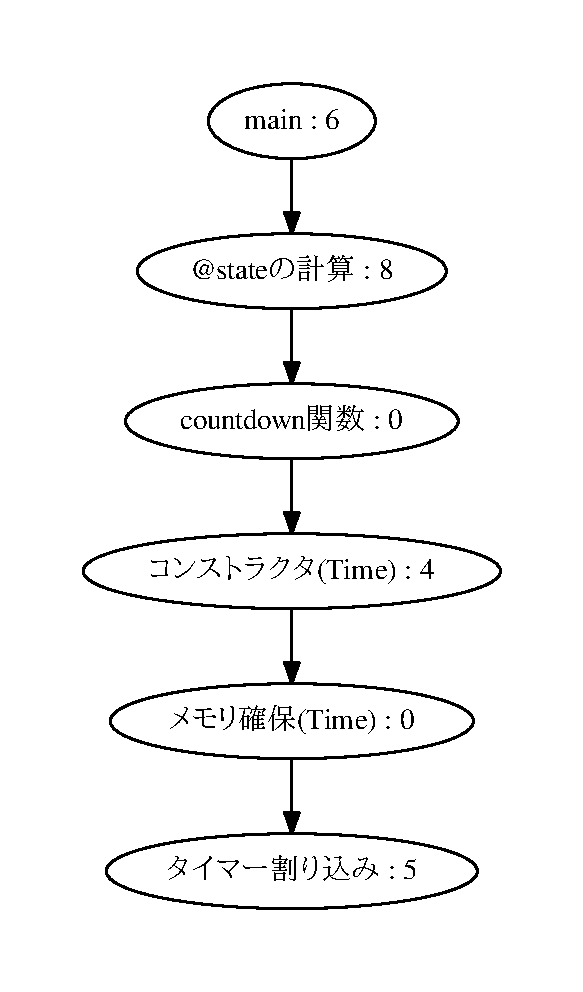
\includegraphics[width=60mm]{figure/call_graph_ktimer.pdf}
 \end{center}
 \caption{スタック使用量が最大となるKTIMERの実行形式の関数コールパス}
 \label{fig:ktimer:call_graph}
\end{figure}

\begin{table}[h]
  \centering
  \begin{tabular}{l|r}
    Programサイズ(avr-sizeコマンドより) & 1858 byte \\ \hline
    Dataサイズ(avr-sizeコマンドより) & 45 byte \\ \hline
    最大スタックサイズ(-fstack-usageオプションおよび手計算により算出)  & 43 byte \\ \hline
  \end{tabular}
\caption{KTIMERのメモリ使用量}
\label{fig:ktimer:size}
\end{table}

\subsection{速度性能}
\ref{sec:implementation:performance:speed}項と同じ手法を用いて速度性能の計測を行うために、
Code \ref{code:ktimer:sfrp:bench}に示す記述をCode \ref{code:ktimer:sfrp}の末尾に追記する。
これにより、KTIMERの\texttt{PB7}番のI/Oポートを観測することによってイテレーション10000回当りの所要時間を求めることができる。

計測の結果は表\ref{fig:ktimer:time}に示す通りとなった。
イテレーション10000回に要する時間はBLINKLEDのそれと比べて約10倍であり、
イテレーション1回の所要時間は約3ミリ秒となることが分かる。
3ミリ秒という値はヒューマンインターフェースの反応時間としては十分であり、KTIMERは問題なく動作することができる。

\lstinputlisting[basicstyle=\ttfamily\small,language=SFRP,tabsize=2,caption={処理時間を計測するための追加記述},label={code:ktimer:sfrp:bench}]{./code/case-study/bench.sfrp}

\begin{table}[h]
  \centering
  \begin{tabular}{l|r}
    一時停止状態で動作させた場合 & \input{code/case-study/evaluation_wait/result1.txt} ミリ秒 \\ \hline
    カウントダウン状態で動作させた場合 & \input{code/case-study/evaluation_tick/result1.txt} ミリ秒 \\ \hline
  \end{tabular}
\caption{KTIMERのイテレーション10000回あたりの所要時間}
\label{fig:ktimer:time}
\end{table}
